\subsection{Round-Robin-Datenbanken}
Round-Robin-Datenbanken sind nicht mit bekannten Datenbanksystemen vergleichbar, da sie in einem proprietären, binären Dateiformat vorliegen.
Daher scheidet der Zugriff per SQL, Texteditor oder über einen Netzwerkport aus.
Um auf Round-Robin-Datenbanken zuzugreifen müssen die dafür entwickelten RRD-Tools verwendet werden.
Diese nehmen die aktuellen Messwerte entgegen und schreiben für jeden Messinterval einen Wert in eine Binärdatei.
Aus den gesammelten Datenbestand können dann die Werte visualisiert oder Statistiken erzeugt werden.
Dieser Datenbestand besteht aus sogenannten Round-Robin-Archives.
Dabei handelt es sich um Ableitungen aus den Primärdateien, die mit Hilfe statistischer Auswertungen ermittelt und für die festgelegten Zeitintervalle komprimiert werden.
Die gesamte Anzahl der gespeicherten Datenwerte steht bereits bei der Erzeugung der RRD fest.
Da auch zu Beginn alle Werte mit Platzhaltern aufgefüllt werden, bleibt die Größe einer RRD über die Zeit gleich, siehe Abbildung \ref{rrd-munin}.

\begin{figure}[ht]
	\centering
	   \fbox{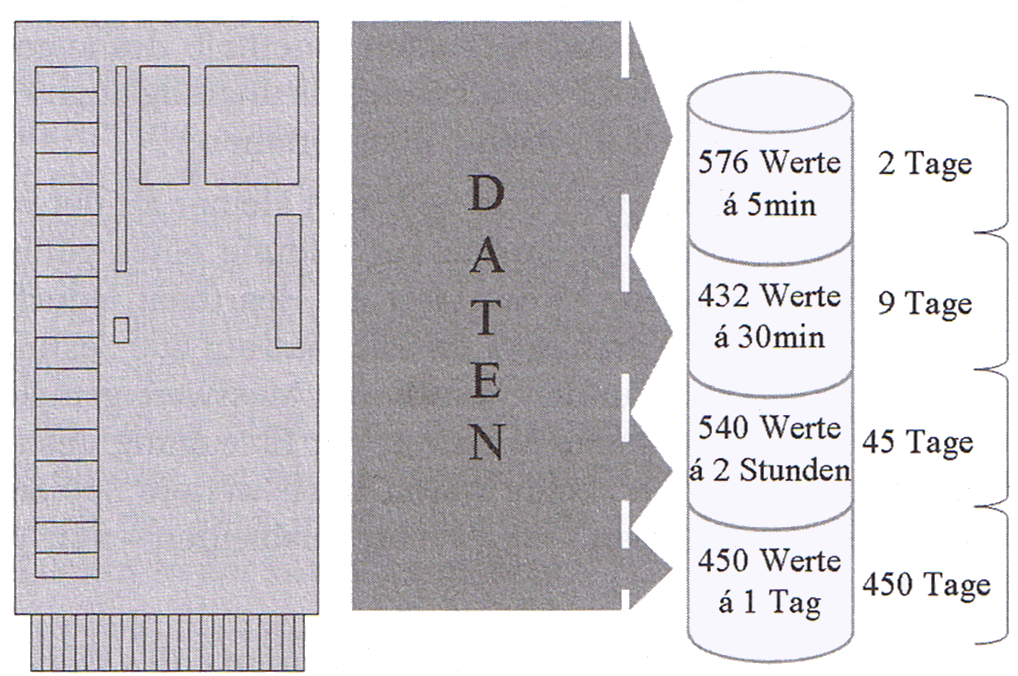
\includegraphics[width=0.76\textwidth]{bilder/rrd.png}}
		\caption[Modell der Round-Robin-Datenbanken]{Modell der Round-Robin-Datenbanken\protect\footnotemark}
		\label{rrd-munin}
\end{figure}
\footnotetext{Quelle: \cite{Mu08} S. 38}

Munin verwendet dieses RRAs als hochauflösende Archive, die die Messwerte des aktuellen Tages, eine etwas komprimierte Fassung zur Darstellung der Daten der laufenden Woche sowie - noch stärker komprimiert - die Daten für den aktuellen Monat und das Jahr enthalten.
%Siehe hierfür Abbildung [?].
Die Komprimierung wird so realisiert, dass Mittelwerte aus der feineren Zeitauflösung errechnet werden und zusätzlich noch spezielle Archivierungsregeln beim Erstellen der RRD-Datei berücksichtigt werden.

Aus diesen Datensätzen mit verschiedenen Zeitauflösungen erstellt Munin automatisch Graphen über die entsprechenden Zeiträume, siehe Abbildung \ref{all4}.

\begin{figure}[ht]
	\centering
	   \fbox{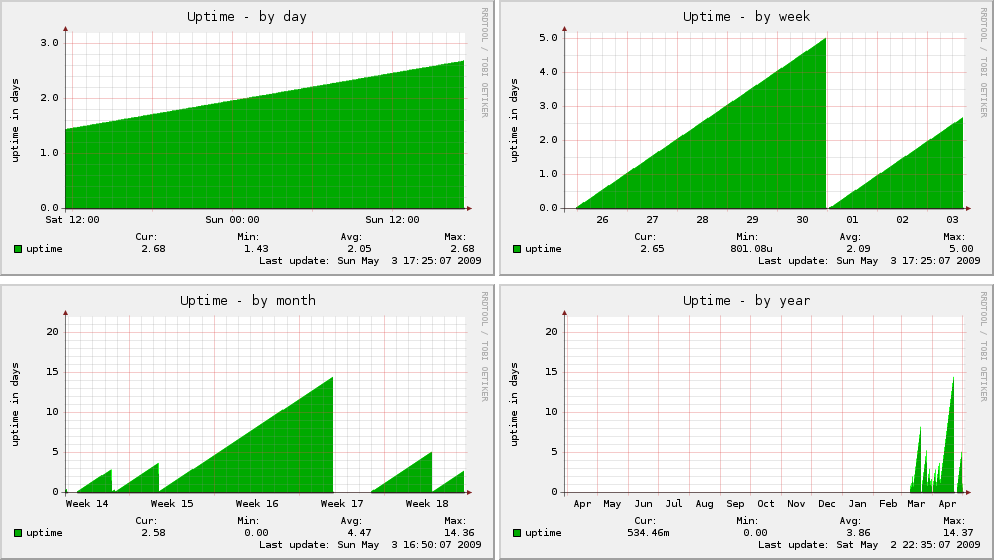
\includegraphics[width=0.95\textwidth]{bilder/all4.png}}
		\caption{Übersicht der \textit{Uptime}}
		\label{all4}
\end{figure}